\documentclass{article}
\usepackage{tikz}
\usetikzlibrary{positioning}

\begin{document}

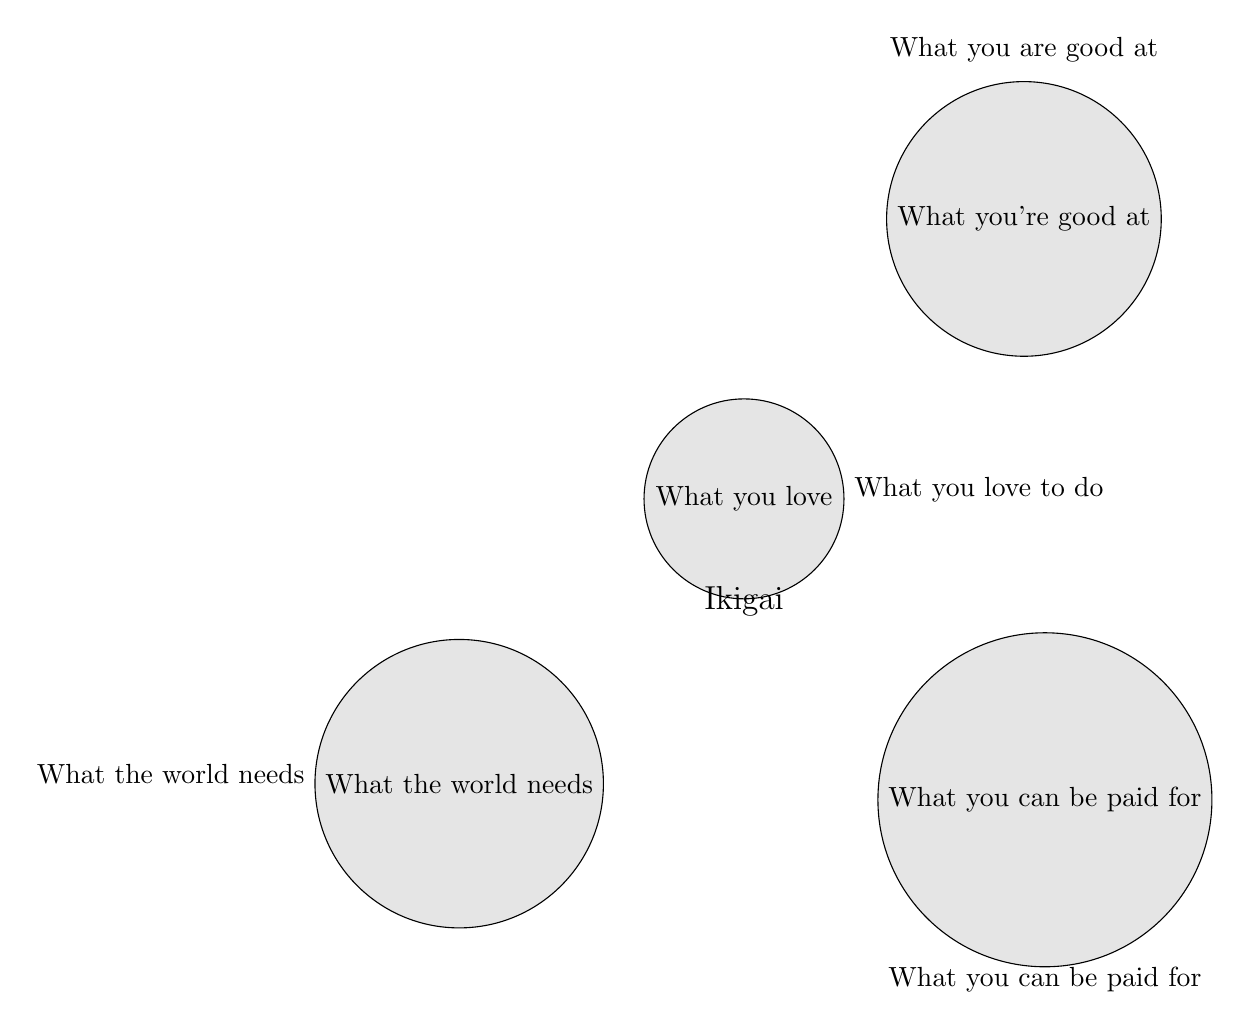
\begin{tikzpicture}[node distance=2cm]

% Circles
\node[draw, circle, fill=gray!20] (what_love) {What you love};
\node[draw, circle, fill=gray!20, above right=of what_love] (good_at) {What you're good at};
\node[draw, circle, fill=gray!20, below right=of what_love] (be_paid) {What you can be paid for};
\node[draw, circle, fill=gray!20, below left=of what_love] (world_needs) {What the world needs};

% Labels
\node[label={[right]What you love to do}] at (what_love.east) {};
\node[label={[above]What you are good at}] at (good_at.north) {};
\node[label={[below]What you can be paid for}] at (be_paid.south) {};
\node[label={[left]What the world needs}] at (world_needs.west) {};

% Title
\node[font=\large] at (0,-1.3) {Ikigai};

\end{tikzpicture}

\end{document}
